\documentclass[9pt,twocolumn,twoside]{../../styles/osajnl}
\usepackage{fancyvrb}
\journal{i524}
\title{Tajo: A Distributed Warehouse System for Large Datasets}

\author[1]{Sagar Vora}

\affil[1]{School of Informatics and Computing, Bloomington, IN 47408, U.S.A.}

\dates{\today}

\ociscodes{HadoopDB, Hive, Distributed, MapReduce, Cluster, Query processing}

% replace this with your url in github/gitlab
\doi{\url{https://github.com/cloudmesh/sp17-i524/raw/master/paper1/S17-IR-2041/report.pdf}}


\begin{abstract}

There has been an increase in the volume of relational data generated
today through a large number of sources. The large volume of data
forces us to find solutions which can cope with them. Recently several
hybrid approaches like HadoopDB, Hive, etc have been introduced to
handle this large data. Although these have been successful in
handling large data, but their architecture makes them inefficient to
handle suboptimal execution strategies. Therefore, in order to solve
the above problem, Apache has developed Tajo, a relational,
distributed data warehouse system on large clusters. It uses Hadoop
Distributed File System (HDFS) for storing data and has its own query
execution engine instead of the MapReduce framework. \newline
\end{abstract}

% \setboolean{displaycopyright}{true}

\begin{document}

\maketitle

\section{Introduction}
In this Big Data era, Hadoop MapReduce
\cite{www-apache-hadoop}\cite{mapreduce-article}, has been used for
processing large-scale data sets. To handle a large amount of data,
several hybrid approaches have been integrated with Hadoop and
parallel databases. However, these cannot avoid the choice of
suboptimal execution strategies because of their architecture, which
led to the development of Tajo. Tajo \cite{www-apache-tajo} is a
relational, distributed data warehouse system which runs on
shared-nothing clusters. It uses Hadoop Distributed File System (HDFS)
as the storage layer and has its own query execution engine instead of
the MapReduce framework. A Tajo cluster consists of one master node
and a number of workers. The master is responsible for the query
planning and coordination among the workers. \newline \newline The
internals of Tajo has three main steps:- \begin{itemize} \item Each
  worker has a local query engine that executes a directed acyclic
  graph (DAG) of physical operators. A DAG of operators can
  accommodate multiple sources of input and can be pipelined within
  the local query engine. Each worker generates query execution plan
  that can employ the existing query evaluation technique
  \cite{query-evaluation-article} \cite{query-processing-article}
  which lie in the database community. \item Tajo can make use of
  various repartition methods specialized for specific
  queries. Consider joining two relations which are already sorted on
  the join key, Tajo needs to repartition only one relation to workers
  in which the corresponding part of another relation resides. \item
  In Tajo, a physical plan that a worker executes is generated in
  runtime according to the available resources like memory, processing
  capability etc. of the workers. Workers can simultaneously execute
  different physical plans in the same phase which allows Tajo to
  maximize the utilization of the resources. \end{itemize}

\section{Advantages of Tajo over MapReduce Hive}
The limitations \cite{tajo-paper} of Hadoop \cite{mapreduce-article}
\cite{hive-paper} MapReduce-Hive technology due to its architecture
led to the development of Tajo. These limitations are as
follows:- \begin{itemize} \item Single Source Input: The join
  operation in relational data warehouses integrates heterogeneous
  data sets from multiple sources. But MapReduce supports only a
  single input source, the join operation is performed by dividing
  input relations through one map reduce job only which doesn't
  produce optimal results. \item Fixed Data Flow: The 3 phases
  \cite{tajo-paper} of MapReduce which are the map, shuffle, and sort
  and reduce. The join operation and aggregation are performed in
  shuffle and sort phase. So it always follows a fixed execution flow
  leaving no room for any optimization needed in the
  processing. Sometimes processing huge datasets need to follow some
  hybrid map reduce flow which is not applicable to the Hadoop
  MapReduce framework. \item Separate Storage: Some hybrid approaches
  \cite{tajo-paper} using the database layer require separate data
  storages for data distribution and processing. The partitioned data
  must be loaded into the database layer for performance benefits. In
  Hadoop, it takes a long time for data loads causing overhead other
  running workloads in the cluster because of a separate data storage
  layer on the HDFS.\end{itemize}

\noindent
Tajo's system architecture has been designed in such a way to overcome
the above shortcomings.


\section{System Architecture}

Figure \ref{fig:architecture} shows the system architecture of Tajo.

\begin{figure}[htbp]
\centering
\fbox{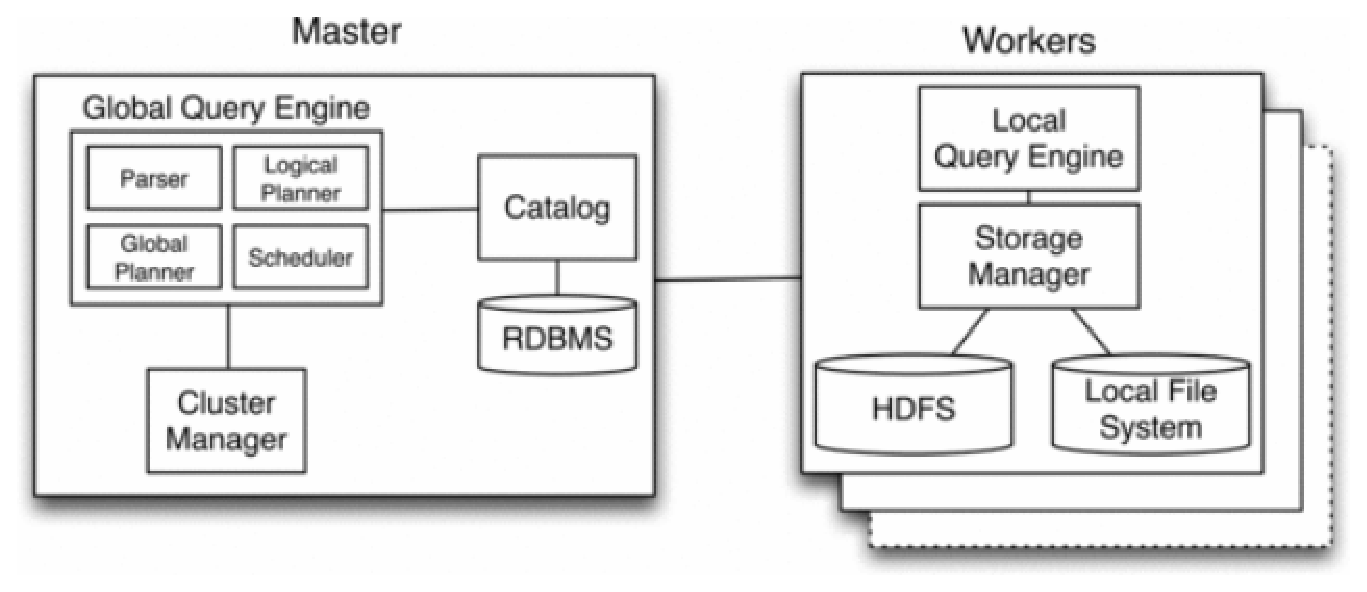
\includegraphics[width=\linewidth]{images/architecture}}
\caption{\cite{tajo-paper} System Architecture of Tajo}
\label{fig:architecture}
\end{figure}

A Tajo cluster \cite{tajo-paper} consists of one master node and a
number of workers. They are connected to one another via high-speed
network. Tajo uses HDFS as the storage layer. HDFS consists of one
name node (master) and a number of data nodes. A Tajo worker and HDFS
data node can run on the same physical machine.

\subsection{Storage Layer}
Tajo uses Hadoop Distributed File System (HDFS)\cite{tajo-paper} as
the basic storage layer. The data in HDFS is distributed automatically
among the cluster nodes. A local query engine of each worker scans
data sets on HDFS. Tajo takes input data from HDFS and later outputs
the results back into HDFS. Tajo even has a local file system and its
storage manager provides interfaces to the operating system. The
physical operators can process data sets on either HDFS or on local
file system.

\subsection{Master}

 The master\cite{tajo-paper} is responsible for planning queries and
 coordinating the activities of workers. The master includes four
 components, cluster manager, catalog, global query engine, and
 history manager. All cluster nodes report their resource information
 like the number of available processors, memory usages, and remaining
 disk spaces periodically to the cluster manager. The catalog
 maintains various metadata, such as tables, schemas, partitions,
 functions, indices, and statistics. Since the metadata are frequently
 accessed by the global query engine, they are stored in a
 conventional RDBMS. The global query engine builds a global plan
 based on the metadata of tables and cluster information which are
 provided from the catalog and the cluster manager, respectively. The
 components of the global query engine will be discussed briefly in
 the Query Processing section. Finally, the history manager records
 the metadata of the executed queries, including query statements,
 statistics, and logical plans.

\subsection{Worker}

A worker has a query execution engine that performs assigned query. A
query unit contains a logical plan and fragments. A fragment is chunk
information of an input relation. During execution, a worker sends
periodically the reports of the running queries and the resource
status to the master which aids in failure. The local query engine
communicates with the storage manager which has its data sets stored
on HDFS and has a local file system storage as well.

\section{Query Processing}
Tajo has an SQL-like query language, called
\cite{www-apache-tajo-tsql} Tajo Query Language (TQL) which supports
most of the SQL commands. In addition to this, TQL also supports two
kinds of variables to indicate a scala value and a temporary table
respectively.

\subsection{Query Planning}

Figure \ref{fig:queryplanning} shows the steps involved in query transformation. 

\begin{figure}[htbp]
\centering
\fbox{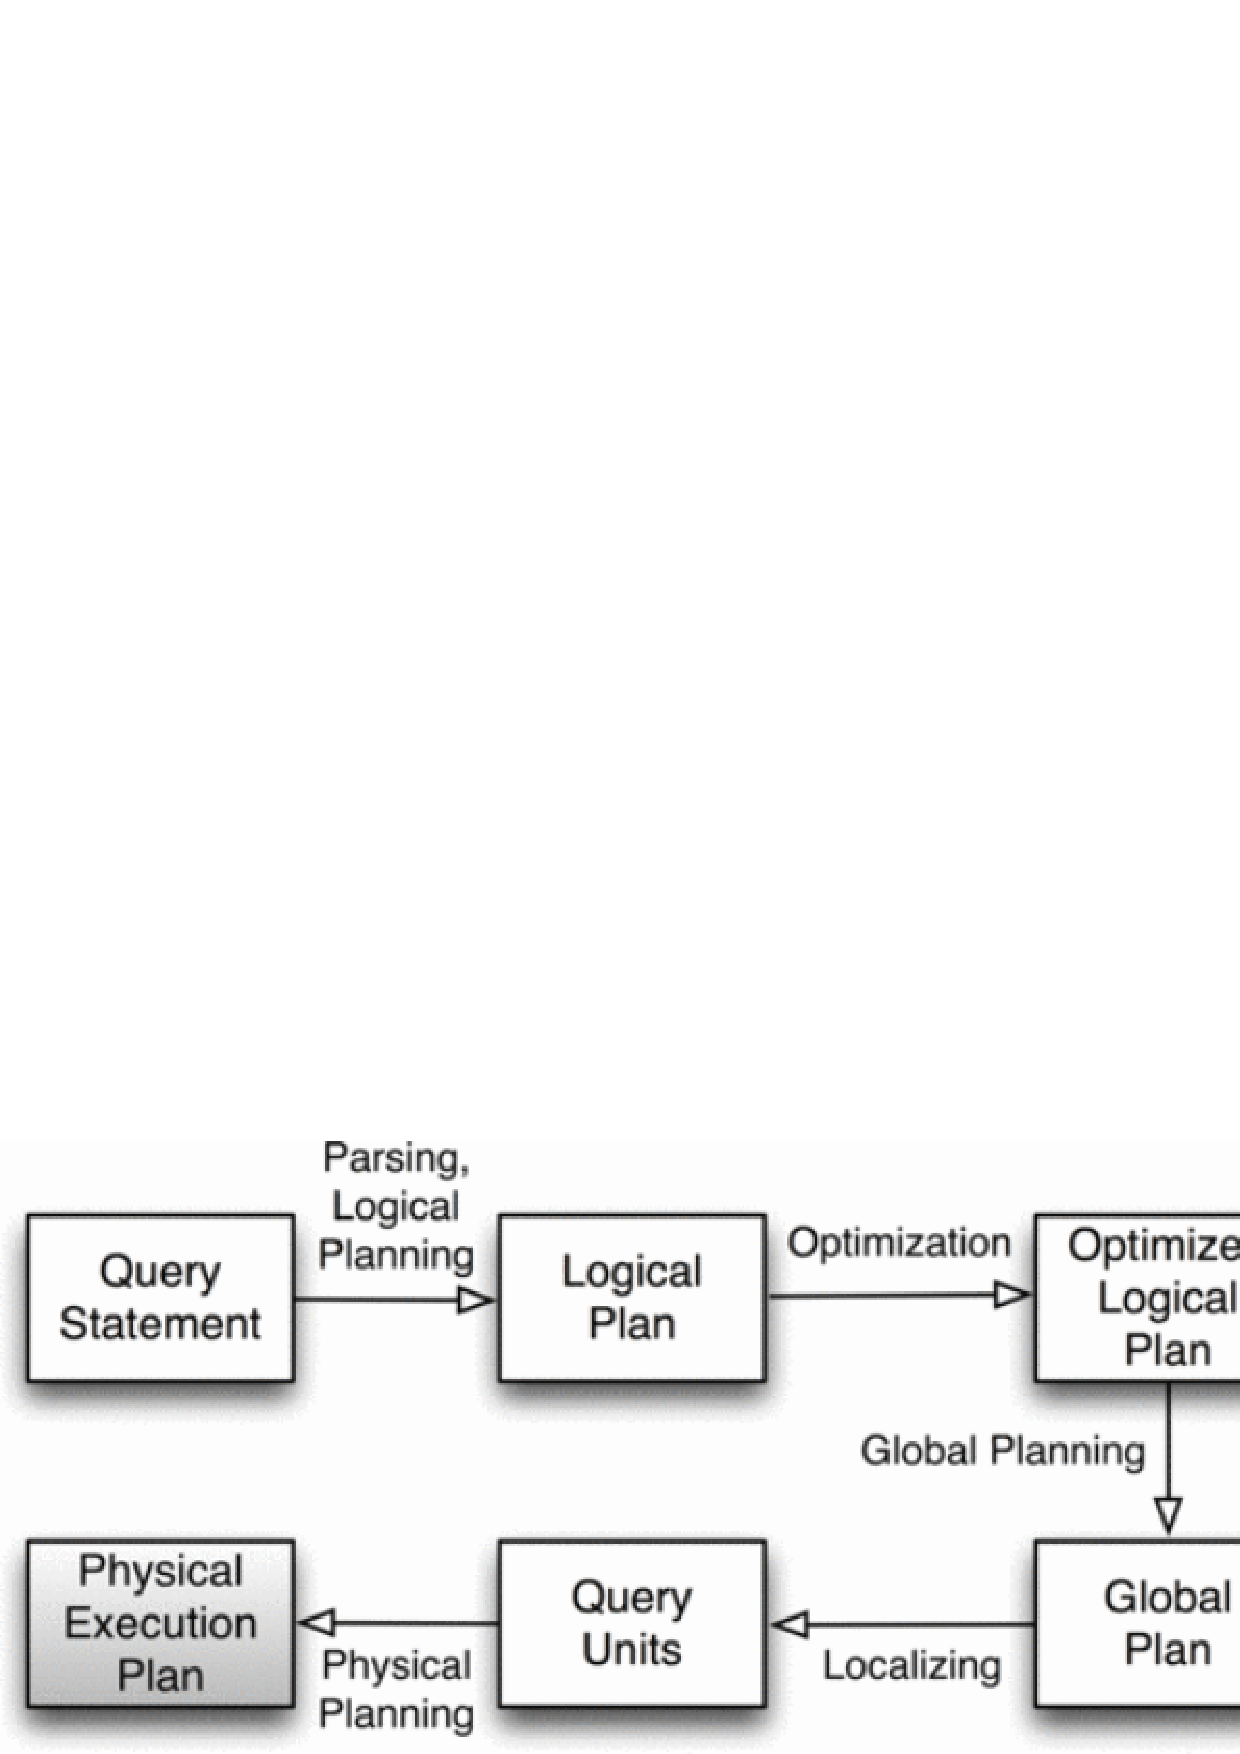
\includegraphics[width=\linewidth]{images/queryplanning}}
\caption{\cite{tajo-paper} Query Transformation}
\label{fig:queryplanning}
\end{figure}

\noindent
In Tajo \cite{tajo-paper} \cite{www-apache-tajo}, it has multiple
steps to transform a query statement to physical execution plans. When
a user submits a query, the global query engine parses the query into
an abstract syntax tree and compiles it into a logical plan. The query
optimizer finds the best logical plan which is similar to the original
logical plan. This is the optimized logical plan which is transformed
into a global query plan. In this step, some logical operators like
group-by, sort, and join are transformed into two phase with
appropriate repartition methods. Usually, the first phase computes
local data on each node, and the intermediate data are
range-partitioned or hash-partitioned on the specified keys (e.g.,
sort keys, grouping keys). The second phase computes the partitioned
data on each node. As a result, a global query plan forms of a
directed acyclic graph (DAG) of subqueries, which represents a data
flow.Based on the physical information of the table, a subquery is
localized into a number of query units, each of which is a basic unit
of a query executed by a worker. Then, the global query engine
schedules the query units along with the DAG of the global
plan.\newline \newline When a worker receives a query unit, it
transforms the logical plan of the query unit into a physical
execution plan according to its own computing resources (e.g.,
available memory). As a result, the query units of the same subquery
can lead to different physical execution plans on different workers.

\subsection{Query Execution}
For input and output of data \cite{tajo-paper}, Tajo has scanners and
appenders. A scanner reads input data from HDFS or local file system,
whereas an appender writes output data to either of them. In the
current implementation, the scanners/appenders of Tajo support CSV and
row-based binary file formats. Since a worker executes a DAG of
physical operators and Tajo can use various repartition methods, it
can do more optimized and efficient query processing.

\section{Experiment}


\begin{figure}[htbp]
\centering
\fbox{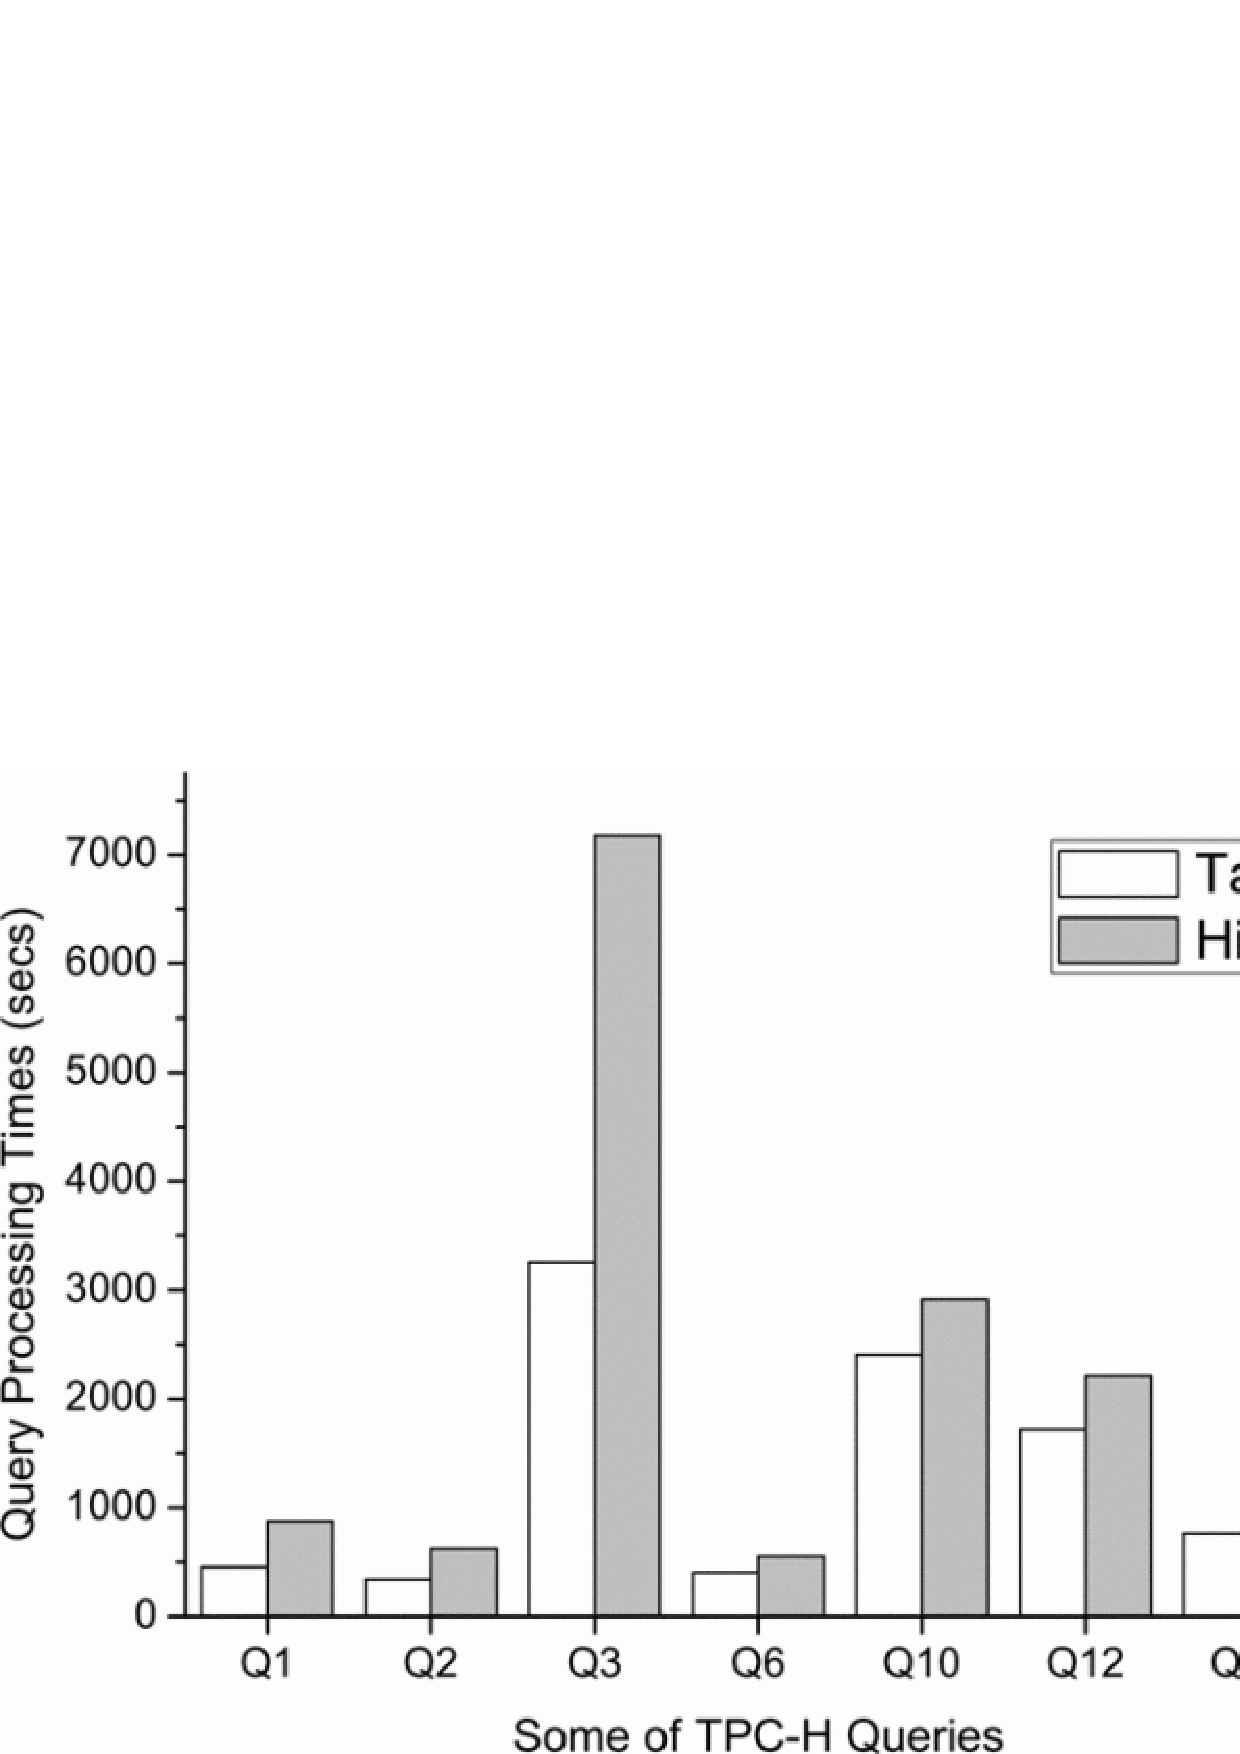
\includegraphics[width=\linewidth]{images/experiment}}
\caption{\cite{tajo-paper} Performance Evaluation using TPC-H}
\label{fig:experiments}
\end{figure}

\noindent
In \cite{tajo-paper}r, the performance of Tajo and Hive has been
compared by using 1TB TPC-H benchmark set. Figure
\ref{fig:experiments} shows the experimental results. For this
experiment, they have used an in-house cluster of 32 nodes, each of
which is equipped with 16GB RAM, 4TB HDD, and an Intel i5 quad core
CPU. The x-axis means the TPC-H queries and the y-axis indicates the
processing times. The results show that the time take by Tajo to
execute SQL queries is less than Apache Hive on the top of MapReduce.

\section{Tajo Shell}
Tajo provides a shell utility named \cite{www-apache-tajo-tsql}
Tsql. It is a command-line interface where users can create or drop
tables, inspect schema and query tables and can execute other sql
commands.\newline \newline
\noindent
For example: bin/tsql [options] [database name] \newline If a database
name is given, tsql connects to the database at startup time else
connects to default database.

\section{Use cases of Tajo}
\subsection{Data warehousing and analysis}
Korea's SK Telecom firm \cite{www-apache-tajo-tutorialspoint} ran Tajo against 1.7 terabytes worth of data and found
it could complete queries with greater speed than either Hive or
Impala.

\subsection{Data discovery}
The Korean music streaming \cite{www-apache-tajo-tutorialspoint}
service Melon uses Tajo for analytical processing. Tajo executes ETL
(extract-transform-load process) jobs 1.5 to 10 times faster than
Hive.

\section{Conclusion}
So, with the use of \cite{www-apache-tajo} Tajo, efficient data
processing and analysis is possible.It processes data faster than the
MapReduce Hive framework and provides distributed data warehouse
capabilities. By supporting SQL standards and advanced database
techniques, Tajo allows direct control of distributed execution and
data flow across a variety of query evaluation strategies and
optimization opportunities.Lastly, being compatible with ANSI/ISO SQL
standard, JDBC driver and various file formats such as CSV, JSON,
RCFile etc extends its capabilities further.

\section*{Acknowledgements}

I would like to thank my professor Gregor von Laszewski and all the
associate instructors for their constant technical support.

% Bibliography

\bibliography{references}
 


\newpage

\appendix


\end{document}
